\documentclass[usenames,dvipsnames,aspectratio=169]{beamer}
\usepackage[utf8]{inputenc}
\usepackage{amsmath,xfrac}
\usepackage{graphicx}
\usepackage{apacite,natbib}
\usepackage{adjustbox}
\usepackage{booktabs}
\usepackage{amsfonts}
\usepackage{hyperref}
\usepackage{pdflscape}
\usepackage{lscape}
\usepackage{caption, subcaption}
\usepackage{pgfplots}
\usepackage{xcolor}

\hypersetup{
    colorlinks,%
    citecolor=black,%
    filecolor=black,%
    linkcolor=black,%
    urlcolor=black
}   % useful for program listings
\usecolortheme{seahorse}

\title{Minimum Wages and the Spatial Distribution of Informality  \\ \small{Applied Macroeconomics: Micro Data for Macro Models} }
\author{Jose M. Quintero}



\AtBeginSection[]
{
  \begin{frame}<beamer>
    \frametitle{Outline}
    \tableofcontents[currentsection]
  \end{frame}
}

\AtBeginSubsection[]
{
   \begin{frame}
        \frametitle{Outline}
        \tableofcontents[currentsubsection]
   \end{frame}
}



\begin{document}

\begin{frame}
  \titlepage
\end{frame}

\begin{frame}{Informality and Min. Wage}
    \begin{figure}
        \begin{center}
        \begin{subfigure}[b]{0.47\textwidth}
            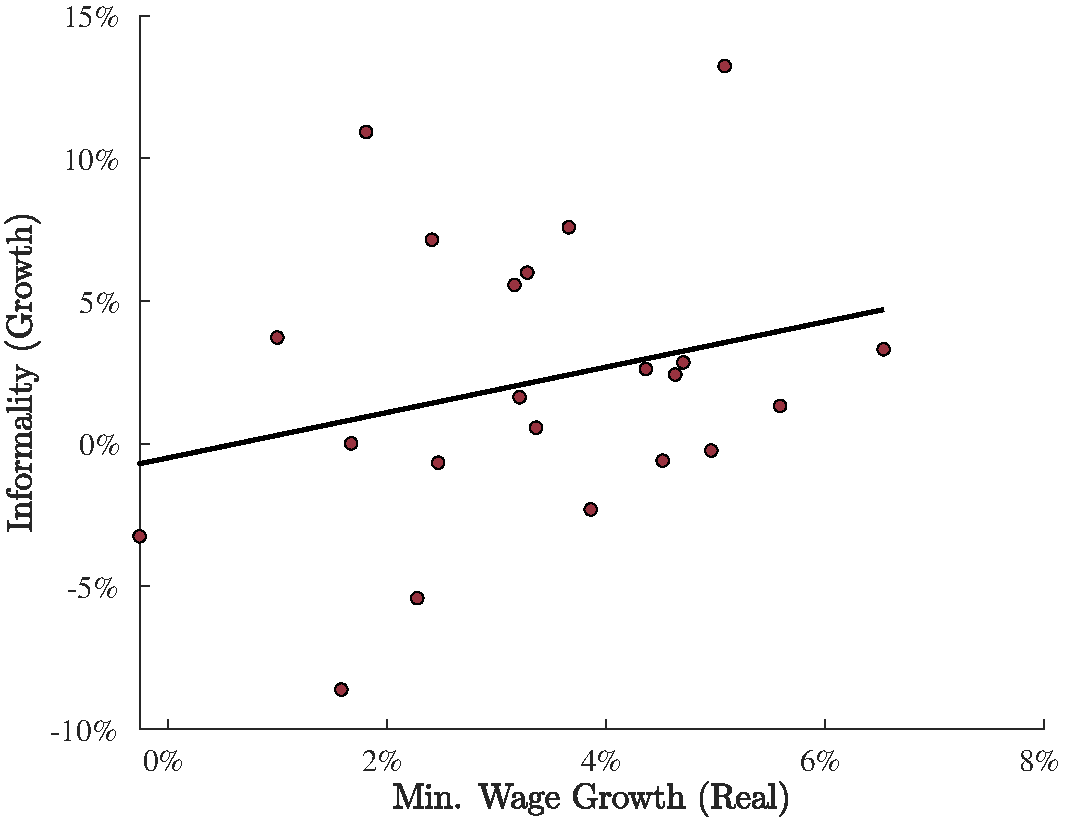
\includegraphics[width=\textwidth]{Figures/infWage_g.pdf}
            \caption{Informality Growth}
        \end{subfigure}
        \begin{subfigure}[b]{0.47\textwidth}
            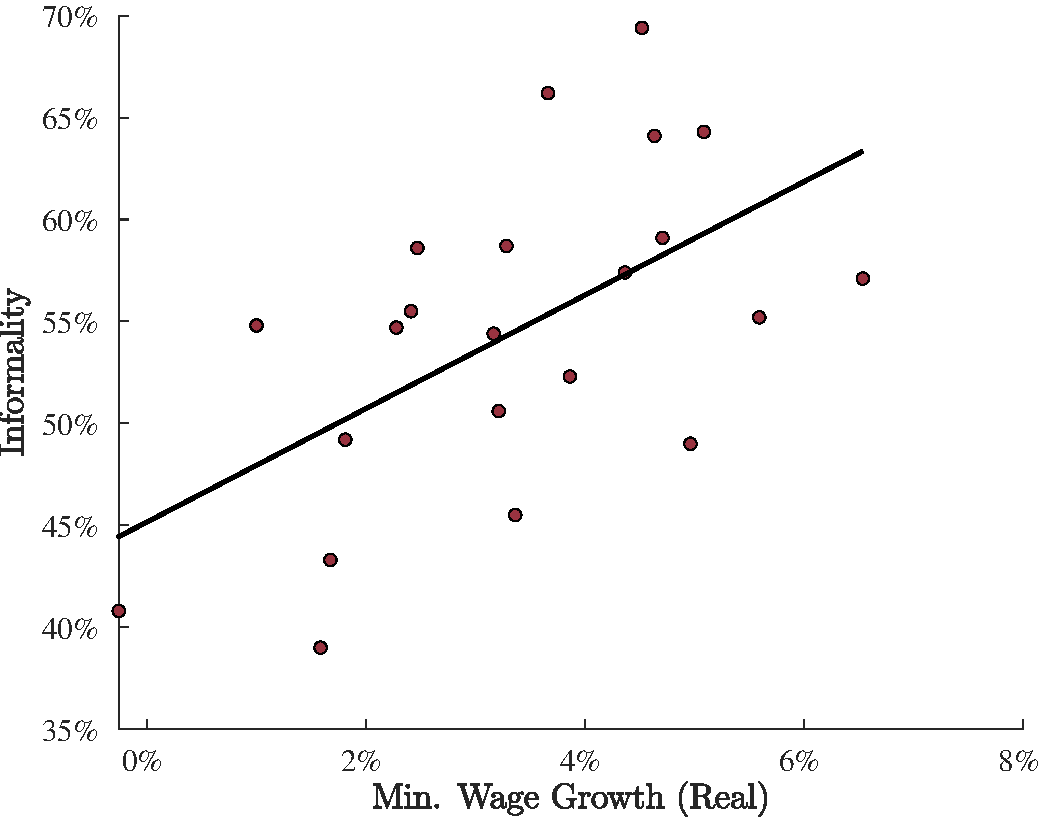
\includegraphics[width=\textwidth]{Figures/infWage_static.pdf}
            \caption{Informality Rate}
        \end{subfigure}
        \end{center}
        \vspace{5pt}
        \tiny{Source: Authors calculations. Panel (a) shows the informality growth rate and how it responds to the growth of minimum wage in real terms.}
    \end{figure}
    \hyperlink{hw1:institution}{\beamerbutton{Institutional Setting}}
\end{frame}

\begin{frame}{Why is this relevant?}\label{hm1:relevance}
\begin{itemize}
    \item Labor informality is a common trait of developing economies. 
        \begin{enumerate}
            \item 20\% - 80\% of labor force is informal in developing countries \citet{Ulyssea20}. 
            \item Unproductive firms can compete against more productive firms by avoiding regulations. 
            \item It provides flexibility towards large entry costs and other distortions. 
        \end{enumerate}
        \bigskip 
        \item Minimum wages at the national is a typical policy instrument in developing countries
        \begin{enumerate}
            \item Ensures minimum level of consumption 
            \item It makes hiring in the formal sector more expensive $\rightarrow$ Informal firms not subject to minimum wage.
        \end{enumerate}
\end{itemize}      
\end{frame}
\begin{frame}{Research Agenda}
\begin{itemize}
    \item Empirical exercises
    \begin{enumerate}
        \item \textbf{Firm Sorting:} Is average firm productivity correlated with informality? Average firm size? Firm Age? Labor productivity?
        \item \textbf{Labor Force:} Are migration flows related to (real) increases in minimum wages? Who is moving and where?  
    \end{enumerate}
    \bigskip 
    \item Build GE model
    \begin{enumerate}
        \item \textbf{Ingredients:} Firms (het.), workers, locations. 
        \item \textbf{Trade-off:} Higher wages $\Rightarrow$ \\
         $\uparrow$ informality + $\downarrow$ average wage. 
        \item \textbf{Calibrate + counterfactual:} Match the model to the data + Explore alternative policies. 
    \end{enumerate}
\end{itemize}
\end{frame}

\begin{frame}{Related Literature}
\begin{enumerate}
    \item \textbf{Labor Informality:} \citet{Ulyssea18}, \citet{DixCarneiro21}
    \begin{itemize}
        \item Causes and consequences of informal labor and informal firms. 
        \smallskip
        \item \textcolor{blue}{This paper:} spatial variation of labor informality. 
    \end{itemize}
    
    \bigskip
    
    
    \item \textbf{Local Labor Markets:} \citet{Bilal20}, \citet{Davis19}
     \begin{itemize}
        \item Effect of externalities and/or frictions on wage premia.
        \smallskip
        \item \textcolor{blue}{This paper:} informal labor markets generate within-city and between-cities earnings inequality. 
    \end{itemize}
    
    \bigskip

    \item \textbf{Minimum Wage:} \citet{Engbom21}, \citet{Berger21}.
    \begin{itemize}
        \item Effect of minimum wage on welfare, employment and earnings. 
        \item \textcolor{blue}{This paper:} effect of national minimum wage on labor informality at the local level.
    \end{itemize}
\end{enumerate}
\end{frame}


\begin{frame}
    \begin{center}
        \textbf{\Huge{Thank You}}
    \end{center}
\end{frame}

\begin{frame}{References}
    \bibliographystyle{apacite}
    \bibliography{references}
\end{frame}



\begin{frame}{Institutional Setting}\label{hw1:institution}
\begin{itemize}
    \item Colombia's economy as a natural experiment for understanding the geography of informality.
    \begin{enumerate}
        \item Colombia labor informality is 50\%. 
    \end{enumerate}
    \item Every year legal minimum wage increases
    \begin{enumerate}
        \item Bargaining between government, firms, and workers. 
        \item The increase in minimum wage considers inflation, economic growth, and worker productivity.
        \item Growth in minimum wages determines other economic variables. 
    \end{enumerate}
    \item Increases in the minimum wage at the national level do not account for local economic trends. 
\end{itemize}
\hyperlink{hw1:motFigs}{\beamerbutton{Back}}
\end{frame}



\end{document}

